\section{Architecture}
\TODO{Add architecture}

\begin{figure}[H]
    \centering
    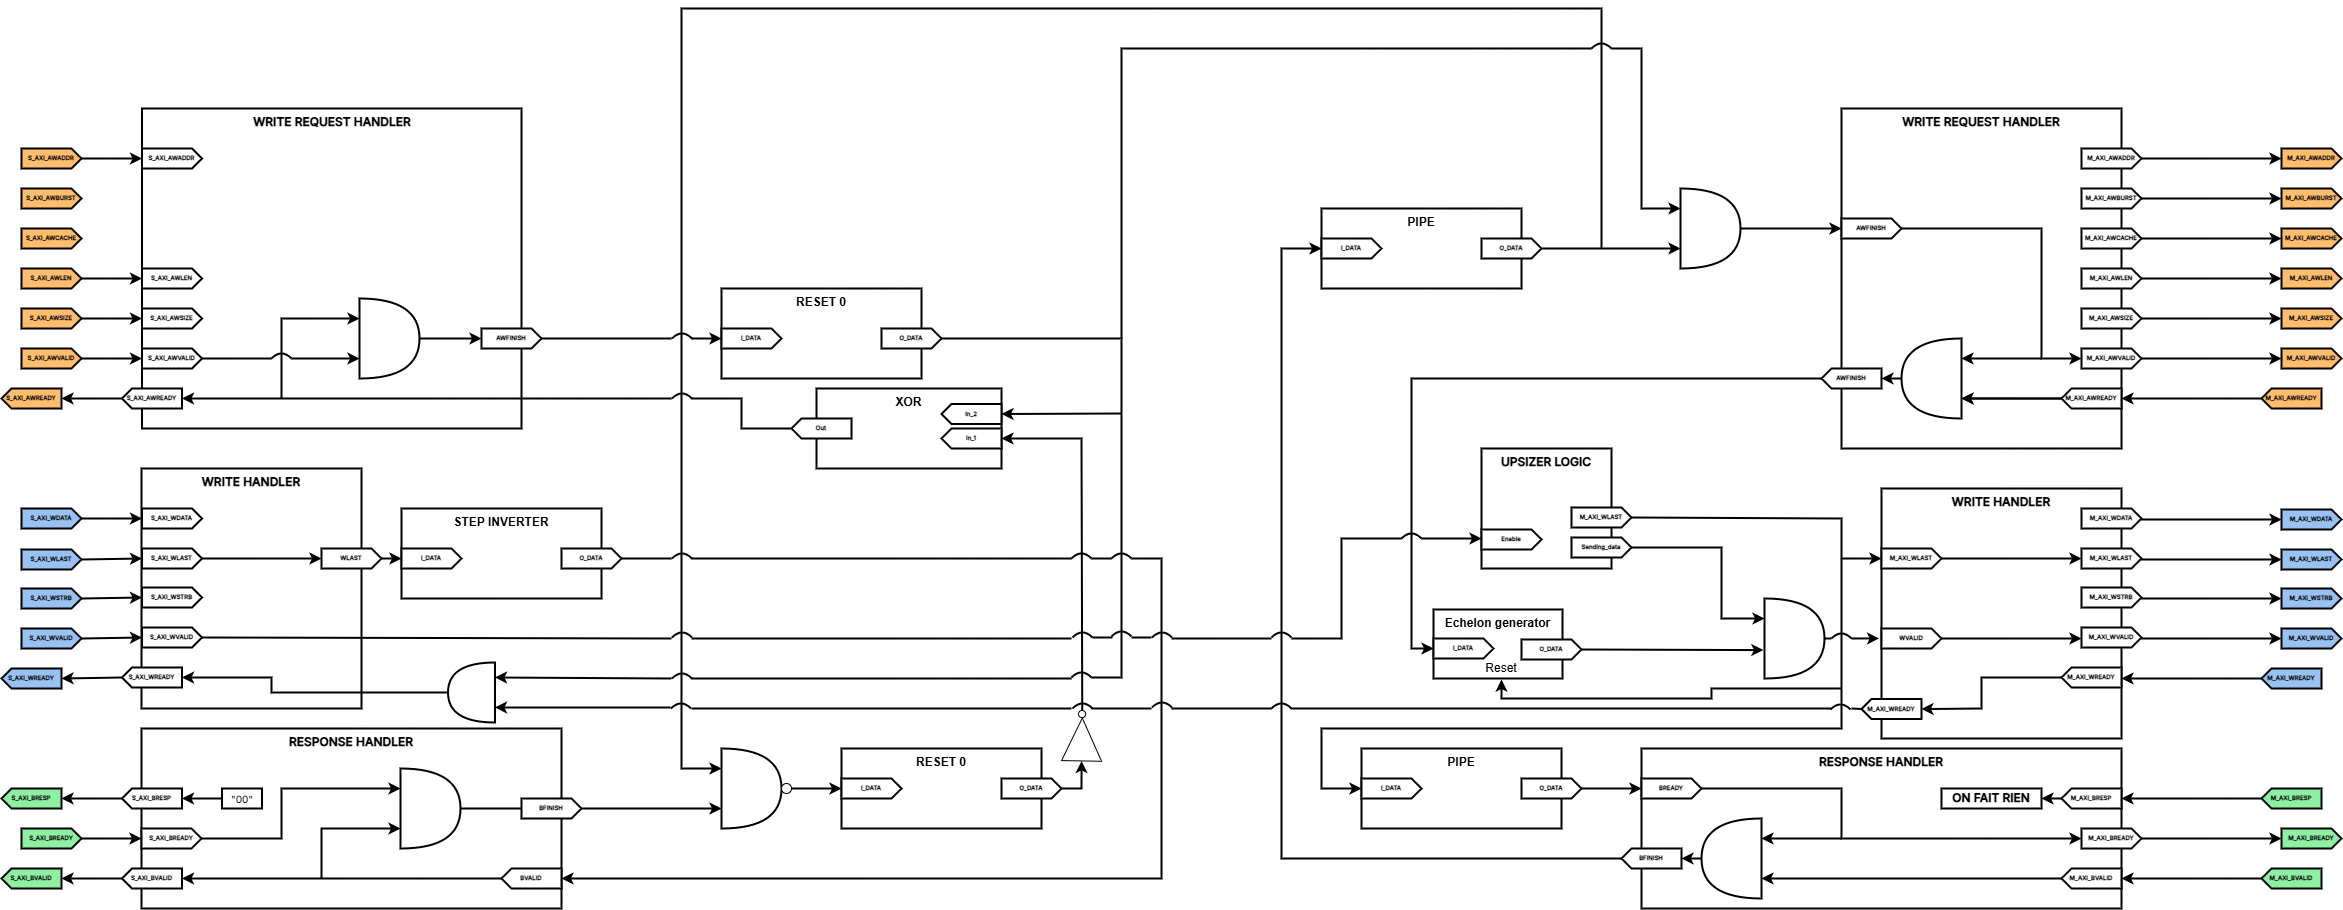
\includegraphics[width=\linewidth]{images/architecture_handshacke.png}
    \caption{Handshake Architecture}
\end{figure}

\begin{figure}[H]
    \centering
    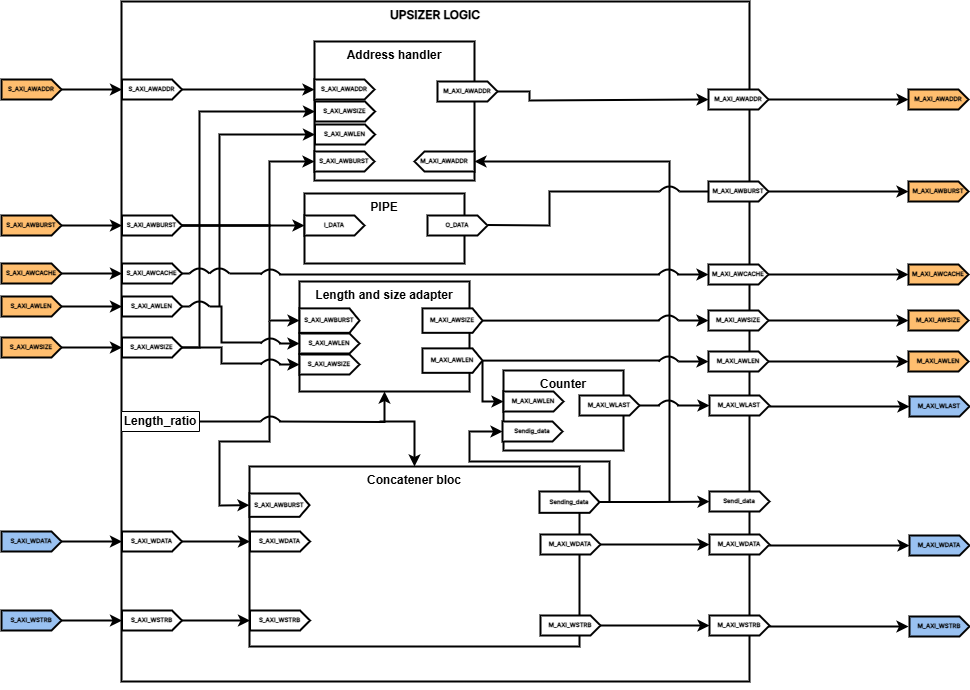
\includegraphics[width=\linewidth]{images/upsizer_logiquee.png}
    \caption{Upsizer logic architecture}
    \label{fig:enter-label}
\end{figure}

\color{red}Note: These architectures are theoritical and have not been verified yet.\color{black}

\subsection{Xilinx IP}

We used the xilinx IP to help us design the Upsizer, and understand the AXI transaction protocol.

\subsection{Address Handler}

On s'est rendu compte que seule l'adresse de départ est envoyée. Lorsque on incrémente l'adresse elle se répercurte en sortie mais elle n'est pas envoyée avec un signal valide donc bizarre car la doc insiste sur cette incrémentation. Peut etre pas a nous de gérer mais le slave en bout de chaine ?

Mais peut etre utile en cas de longeur de transfert tres importante coté lecture puisque le nombre de transfert va etre multiplier par 4.

Finalement on pense que dans le cas de l'upsizer, ca ne sera jamais un probleme

\subsection{Write Transaction}

On observe bien le changement de la size en écriture et de la length

\subsection{Read Transaction}
On observe pas le changement de la size en lecture et de la length, ce qui est très etrange et me laisse perplexe


\newpage

\subsection{Length \& Size Manager}
\begin{itemize}
    \item Burst Mode Fixed
\end{itemize}
\code{aXlen} and \code{aXsize} pass through and are not modified. 

\begin{table}[H]
\begin{threeparttable}
\caption{Burst mode FIXED example}
\begin{tabularx}{\linewidth}{X | X  || X | X}
\hline
\textbf{Master Size}   & \textbf{Master Length} & \textbf{Slave Size}   & \textbf{Slave Length} \\ 
\hline        
32 bits \newline (\texttt{aXsize = 2}) & 4 transferts \newline (\texttt{aXlen = 3}) & 32 bits \newline (\texttt{aXsize = 2}) & 4 transfers \newline (\texttt{aXlen = 3}) \\
\hline

32 bits \newline (\texttt{aXsize = 2}) & 8 transferts \newline (\texttt{aXlen = 7}) & 32 bits \newline (\texttt{aXsize = 2}) & 8 transfers \newline (\texttt{aXlen = 8}) \\
\hline
\end{tabularx}
\end{threeparttable}
\end{table}

In this exemple, \code{Xstrb} indicates that only the first 4 bytes are valid.

\begin{itemize}
    \item Burst Mode Incr et Wrap
\end{itemize}
\code{aXlen} is divided by \code{SIZE_RATIO} and \code{aXsize} is multiplied by \code{SIZE_RATIO}.

\begin{table}[H]
\begin{threeparttable}
\caption{Burst mode INCR and BURST example}
\begin{tabularx}{\linewidth}{X | X  || X | X}
\hline
\textbf{Master Size}   & \textbf{Master Length} & \textbf{Slave Size}   & \textbf{Slave Length} \\ 
\hline        
32 bits \newline (\texttt{aXsize = 2}) & 4 transferts \newline (\texttt{aXlen = 3}) & 128 bits \newline (\texttt{aXsize = 4}) & 1 transfer \newline (\texttt{aXlen = 0}) \\
\hline

32 bits \newline (\texttt{aXsize = 2}) & 8 transferts \newline (\texttt{aXlen = 7}) & 128 bits \newline (\texttt{aXsize = 4}) & 2 transfers \newline (\texttt{aXlen = 1}) \\
\hline
\end{tabularx}
\end{threeparttable}
\end{table}
    



Option TLAST => Instantiation use LAST \\
Divise length par Ratio(Bus sortie/Bus entrée)




En mode Fixed, les données sortent à chaque coup d'horloge avec une taille de 128 bits. Le strb indique que seul les 4 premiers bytes sont valides dans les 16 du mot de 128 bits. D'ailleurs le mot de 128bits est composé du signal envoyé par le maître concaténer Ratio fois. AWSIZE est propagé du coté maitre au coté esclave. Length reste constant. Le strobe est egalement propagé avé des zéros devang.

En mode Incr ou Wrap, le mot est composé de la concaténation des données envoyées par le maitre. AWSIZE augmente pour atteindre la taille du bus esclave. Length est divisé par le ratio. Le strb est concaténé également et reseté comme les données à la fin du transfert coté slave.

\subsection{Concatenator}

\subsection{Handshake Note}

Le \code{S_AWREADY} après la première transaction ne se lève que lorsque le HandShake entre \code{M_AWREADY} et \code{M_AWVALID} est effectué.

\begin{figure}[H]
    \centering
    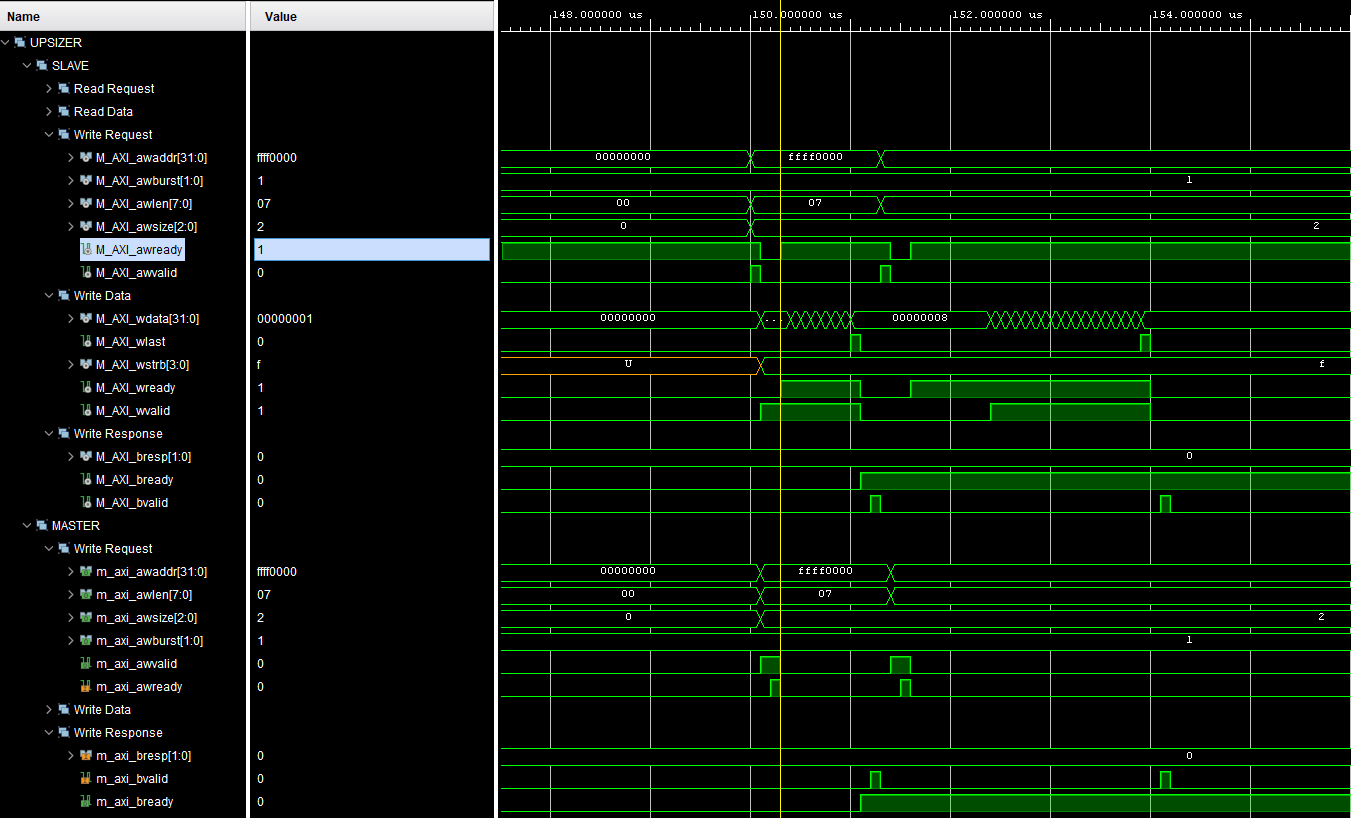
\includegraphics[width=\linewidth]{images/aw_ready_condition.PNG}
    \caption{Handshake AWREADY}
\end{figure}

Le signal \code{S_WREADY} passe à l'état bas après 4 données envoyées si la donnée de 128 bits sur le canal \code{M_WDATA} n'a pas été envoyée.

\begin{figure}[H]
    \centering
    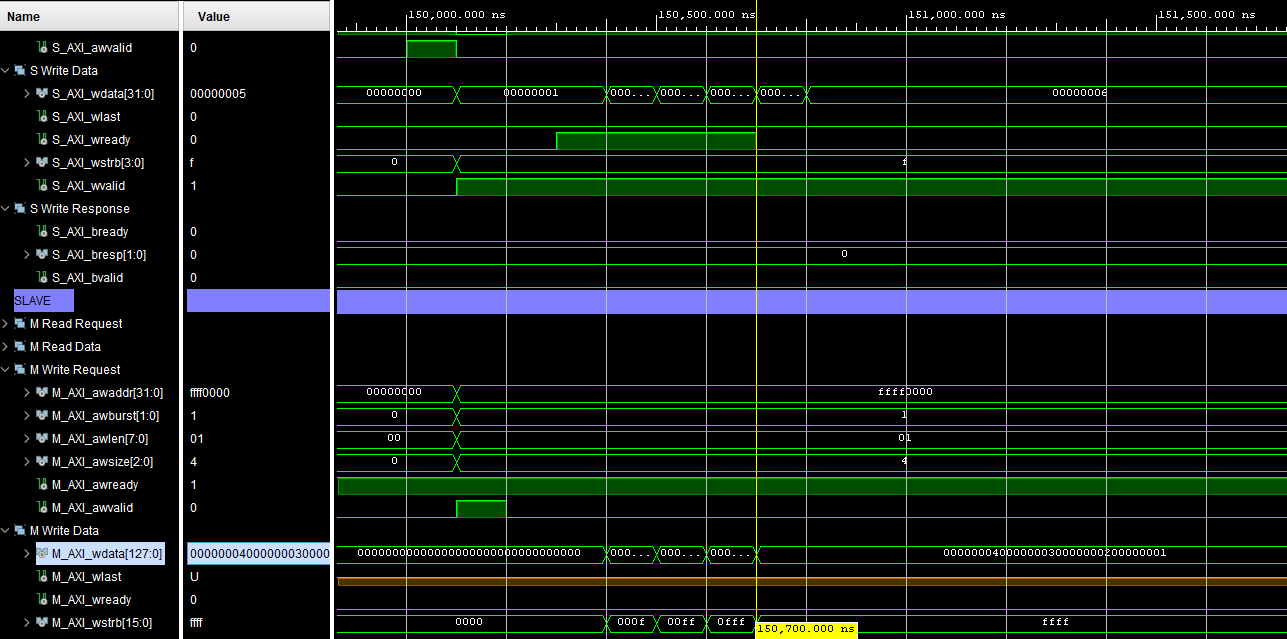
\includegraphics[width=\linewidth]{images/w_ready_condition.PNG}
    \caption{WREADY}
\end{figure}